\documentclass{article}
\usepackage{hyperref}
\usepackage[utf8]{inputenc}
\usepackage{amsfonts}
\usepackage{amsmath}
\usepackage{amssymb}
\usepackage{tikz}
\usepackage{bbm}
\usepackage{relsize}
\usepackage{pgfplots}
\usepackage{scalerel}
\usepackage{wrapfig}
\usepackage[T1]{fontenc}       % change font encoding to T1
\usepackage[framed,numbered]{matlab-prettifier}
\pgfplotsset{width=10cm,compat=1.9}
\addtolength{\oddsidemargin}{-.875in}
	\addtolength{\evensidemargin}{-.875in}
	\addtolength{\textwidth}{1.75in}

	\addtolength{\topmargin}{-.875in}
	\addtolength{\textheight}{1.75in}

\title{Meccanica Razionale Riassunti}
\author{Simone Paloschi}
\date{terzo Anno primo Semestre INGMTM}
\linespread{1.5}

\begin{document}

%Lezione 1
\section{Cinematica}


\subsection{Cinematica del Punto Materiale}
%
\textbf{Spazio delle configurazioni} di un punto materiale in $d\in\mathbb{N}$ dimensioni è lo spazio euclideo di dim d: $\mathcal{E}_d$ \\ \\
%
%
%
\textbf{Spazio vettoriale} è un insieme V con 2 proprietà: \ \ \
• : $V\times\mathbb{R}\rightarrow V$ \ \ \ \ + : $V+V\rightarrow V$ \ \ Allora:\\
\ - (V,+) è detto gruppo algebrico\\
\ - Se dimV = n allora  $\ \ \ \{\overline{u}_1,...,\overline{u}_n\}$ linearmente indipendenti è una base di V \\
\ - Data la base, \ \ $\forall \overline{z} \in V \ \ \exists! \ \alpha_1 ... \alpha_n \in\mathbb{R} \ \ t.c. \ \ \overline{z}=\sum_{j=1}^n\alpha_j\overline{u}_j$\\ \\
%
%
%
\textbf{Prodotto scalare} : $\mathbb{R}^n \times\mathbb{R}^n\rightarrow\mathbb{R}$ \ \ \ \ $\overline{u} \cdot \overline{v} \ = \ \sum^n_{j=1}u_jv_j$ \\
\textbf{Prodotto vettoriale} : $\mathbb{R}^3 \times\mathbb{R}^3\rightarrow\mathbb{R}^3$ \ \ \ \ $(\overline{u} \wedge \overline{v})_i \ = \ \sum^3_{j,k=1}\varepsilon_{ijk}\ u_jv_k$ \ \ e valgono:\\
\ • \ \ $\overline{u} \wedge \overline{v} \ = \ \
\begin{vmatrix}
\hat{i} \ \ \ \hat{j}  \ \ \ \hat{k} \\
u_1 \ u_2 \ u_3 \\
v_1 \ v_2 \ v_3 \\
\end{vmatrix}$ \\
\ • \ \ $\overline{u} \wedge \overline{v} \ = \ - \overline{v} \wedge \overline{u}$\ \ (è anticommutativo) \\
\ • \ \ $\overline{u} \wedge (\overline{v} \wedge \overline{w}) \ \neq \ (\overline{u} \wedge \overline{v}) \wedge \overline{w}$ \ \ (non è associativo)\\
\ • \ \ $\overline{u} \wedge (\overline{v} \wedge \overline{w}) \ = \ (\overline{u}\cdot\overline{w})\overline{v} - (\overline{u}\cdot\overline{v})\overline{w}$\ \ (+dim) \\
\ • \ \ $(\overline{u}+\overline{v})\wedge \overline{w} \ = \ \overline{u}\wedge \overline{w} + \overline{v}\wedge\overline{w}$ \ \ (è distributivo)  \\ \\
%
%
%
\textbf{Modulo di un vettore} : $|\overline{u}| \ = \ \sqrt{\overline{u}\cdot\overline{u}} $ \ \ valgono: \\
\ • \ \ $\overline{u}\cdot\overline{v} = |\overline{u}||\overline{v}|cos\theta $ \\
\ • \ \ $\overline{u}\wedge\overline{v}=|\overline{u}||\overline{v}|sen\theta$ \\ \\
%
%
%
\textbf{Spazio euclideo} $\mathcal{E}_d$ è un insieme di punti $\mathcal{E}_d$ e un'applicazione A: $\mathcal{E}_d\times\mathcal{E}_d\rightarrow V$ (spazio vettoriale) t.c. \\
%
\ • \ \ $P,Q \in\mathcal{E}_d \rightarrow \overline{PQ}\in V$ \ \ \ \ \ \ • \ \ $\overline{PQ}=-\overline{QP}$ \\
\ • \ \ $\overline{PQ}+\overline{QR}=\overline{PR}$ \ \ \ \ \ \ \ \ \ \ \ \ • \ \ $\forall P \in \mathcal{E}_d, \forall \overline{u} \in V \ \ \exists! \ Q \in \mathcal{E}_d \ | \ \overline{PQ}=\overline{u}$ \\ \\
%
%
%
\textbf{Osservatore} (o sistema di riferimento) in $\mathcal{E}_d$ è un insieme: $\mathcal{O}= \{O; \hat{e}_1,...,\hat{e}_d \}$ t.c.

$O\in\mathcal{E}_d$ e $ \{\hat{e}_1,...,\hat{e}_d \} $ è un sistema ortonormale in $\mathbb{R}^d$ \\ \\
%
La configurazione del punto materiale P si può assegnare con le \textbf{coordinate} $\overline{n} \in\mathbb{R}^d$ di P rispetto a $\mathcal{O}$ \\
Le coordinate $\overline{x}(t)$ di P rispetto al tempo si possono vedere come:\\
\ • \ \ punto nello spazio-tempo $\mathbb{R}^d\times\mathbb{R}$ che individua la linea di universo di P \\
\ • \ \ funzione $\overline{x}(t): \mathbb{R}\rightarrow\mathbb{R}^d$ è detta \textbf{traiettoria} \ (o moto) \\ \\
%
Data la traiettoria e assunta $\overline{x}(\cdot) \in C^2(\mathbb{R})$ \ \ \ \ \
\textbf{Velocità}: $\overline{v}(t) = \frac{d\overline{x}}{dt}(t)$ \ \ \ \ \ \ \textbf{Accelerazione}: $\overline{a}(t) = \frac{d^2\overline{x}}{dt^2}(t)$

\pagebreak %se lo togli metti \\



%Lezione 2
\subsection{Moto in Coordinate Intrinseche}
%
Sia $\overline{x}(\cdot) \in C^2([t_0,t_1])$ la traiettoria di P. \ Assumendo che $\overline{x}(t)$ abbia solo zeri isolati allora: \\ 
\textbf{s(t) ascissa curvilinea} è la lunghezza dell'arco di curva percorsa tra $t_0$ e t è
\begin{equation*}
    s(t)=\int_{t_0}^t \dot{s}(\tau) d\tau \ = \ \int_{t_0}^t |\dot{\overline{x}}(\tau)| d\tau
\end{equation*}
s(t): $\mathbb{R}\rightarrow\mathbb{R}^+$ anche detta legge oraria del moto del punto, è una funzione monotona crescente.

Di conseguenza s($\cdot$) è invertibile $\implies \exists \ t(\cdot):\mathbb{R}^+\rightarrow\mathbb{R}$ \ t.c. \ s(t($\sigma$)) = $\sigma$ \ e \ $\frac{dt}{ds}(s)= \frac{1}{|\dot{\overline{x}}(t(s))|}\ \ \ \forall t \ |\ \overline{v}(t)\neq \overline{0} $

Possiamo quindi parametrizzare ugualmente le curve con il tempo o con la distanza percorsa

Notazione: $\dot{f}=\frac{df}{dt} \ \ f'=\frac{df}{ds}$ \\ \\
%
%
%
Poste le ipotesi su $\overline{x}(\cdot)$ sono definiti la parametrizzazione $\overline{\gamma}:[0,L]\rightarrow\mathbb{R}^d$ t.c. $\overline{\gamma}(s)=\overline{x}(t(s))$ e i versori:
\ • \ \ \textbf{tangente} \ \ $\hat{\tau}(s) := \overline{\gamma}'(s) $ \\
\ • \ \ \textbf{normale} \ \ $\hat{n}(s):=\frac{\hat{\tau}'(s)}{|\hat{\tau}'(s)|}$\\
\ • \ \ \textbf{binormale} \ \ $\hat{b}(s):=\hat{\tau}(s)\wedge\hat{n}(s)$ \\
Inoltre possiamo definire i seguenti valori: \\
\ • \ \ \textbf{Curvatura} della traiettoria \ \ $k:[0,L]\rightarrow\mathbb{R}^+$ \ t.c. \ $k(s) := |\hat{\tau}'(s)|$\\
\ • \ \ \textbf{Torsione} della curva \ \  $h:[0,L]\rightarrow\mathbb{R}^+$ \ t.c. \ $h(s) := |\hat{b}'(s)|$ \\ \\
%
%
%
Teorema: \ \textbf{Formule di Frenet-Serret} \ \ \ (+dim)\\
\phantom{\ } Sotto le ipotesi di $\overline{x}(\cdot)$ e $\forall s \in [0,L] \ t.c. \ \overline{\gamma}'(s)\neq 0$ \\
\ • \ $\hat{\tau}(s), \hat{n}(s), \hat{b}(s)$ formano una terna ortonormale in $\mathbb{R}^3$ \ \ \ \ \ \ • \
$\begin{cases}
\hat{\tau}'(s)=k(s)\hat{n}(s) \\
\hat{n}'(s)=-k(s)\hat{\tau}(s)+h(s)\hat{b}(s)\\
\hat{b}'(s)=-h(s)\hat{n}(s)
\end{cases}$ \\ \\
Prop: Poste le ipotesi su $\overline{x}(\cdot)$ si ha: \ \ \ \
• $\overline{v}(t)=\dot{s}(t)\hat{\tau}$ \ \ \ \
• $\overline{a}(t)=\ddot{s}(t)\hat{\tau}+k\dot{s}^2(t)\hat{n}$ \ \ \ (+dim)\\




\subsection{Cinematica del Corpo Rigido}
%
\textbf{Corpo Rigido} è un sistema di $N\in\mathbb{N}\cup\{+\infty\}$ punti materiali che soddisfano: \\ $|\overline{OP}_i(t) - \overline{OP}_j(t)|$ = cost   $\forall t \in \mathbb{R} \ \ \forall i,j \in \{1...N\}$ 
\ \ \ ovvero la distanza tra i punti del sistema rimane costante

Per identificare univocamente la configurazione del corpo rigido in 3D per N$\ge$3 servono 3N-6 coordinate. \\ \\
%
%Lezione 3
%
\textbf{Osservatore}, o anche sistema di riferimento, è \textbf{solidale} ad un corpo rigido se le posizioni del corpo 

rispetto a $\theta = \{O',\hat{e}_1, \hat{e}_2, \hat{e}_3 \} $ non dipendono dal tempo. \\
%
Teorema: Un sistema di punti materiali è un corpo rigido se e solo se $\exists \theta$ solidale \ \ \ (+dim) \\
%
Oss: La posizione di un punto nello spazio è assegnata univocamente dalle distanze da 3 punti non collineari. \\ \\
%
Prop: La configurazione di un corpo rigido \textbf{piano} è determinata univocamente da 3 coordinate\ \ \ \ (+dim)\\
%
Prop: Per la configurazione di un C \textbf{tridimensionale} sono necessarie e sufficienti 6 coordinate \ \ \ \ (+dim)\\ \\
%
%
%
Prop: Ogni rotazione in $\mathbb{R}^3$ è rappresentata da una matrice ortonormale $R\in\Theta_3$, \\
\phantom{Prop: }Che equivale al prodotto di 3 rotazioni attorno agli assi $\hat{i}, \hat{j}, \hat{k}$. \ \ \ \ \ \ \ \ \ \ \ \ \ \ \ \ \ \ \ \ \ \ \ \ \ \ \ \ \ \ \ \ \ \ \ \ \ \ \ \ \ \ \ \ \ \ \ \ \ \ \ \
%
%
%
\begin{wrapfigure}{r}{0.15\textwidth}
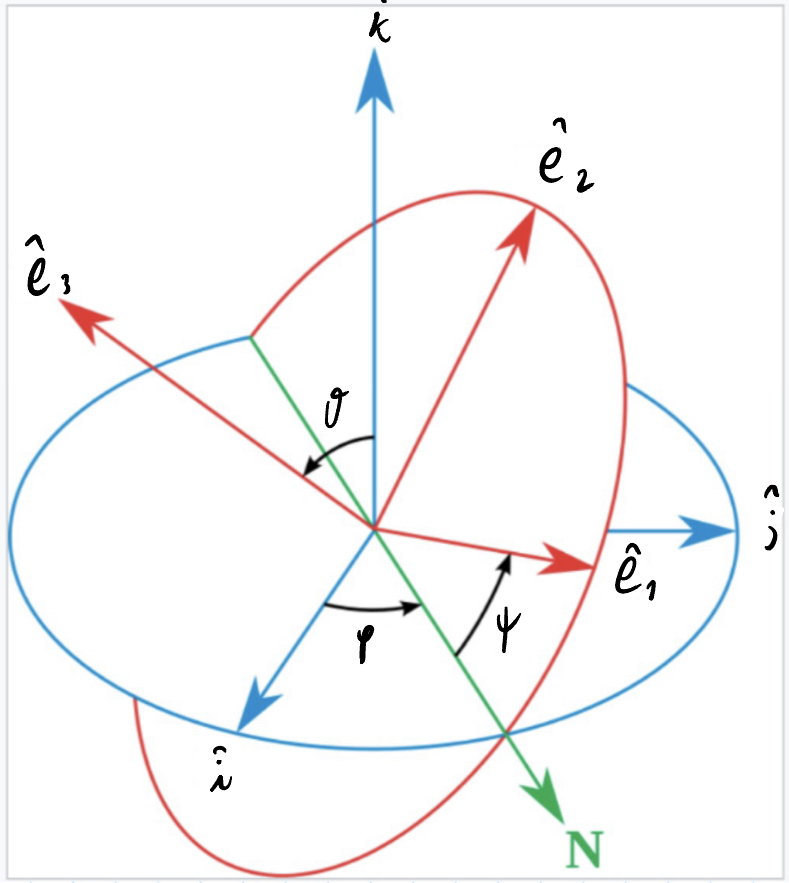
\includegraphics[width=0.15\textwidth]{Eulero.jpeg}
\end{wrapfigure} \\
%
%
\textbf{Angoli di Eulero} sono coordinate angolari che identificano univocamente 

la posizione di un sistema solidale, nell'ipotesi O=O':\\
%
%
\ • \ \ $\theta$ angolo di \textbf{mutazione} $\in [0,\pi]\ :\ cos\theta := \hat{e}_3\cdot\hat{k}$; \\
\ • \ \ $\phi$ angolo di \textbf{precessione} $\in [0,2\pi]\ :\ cos\phi := \hat{i}\cdot\frac{\hat{k}\wedge\hat{e}_3}{|\hat{k}\wedge\hat{e}_3|}$; \\
\ • \ \ $\psi$ angolo di \textbf{rotazione propria} $\in [0,2\pi]\ :\ cos\psi := \hat{e}_1\cdot\frac{\hat{k}\wedge\hat{e}_3}{|\hat{k}\wedge\hat{e}_3|}$;\\ \\
%
%
%
Prop: Vale sempre, per un corpo rigido: \ $(\overline{V}_P-\overline{V}_Q)\cdot\overline{QP} = 0$ \ \ \ dove \ $\overline{QP}=\overline{X}_P-\overline{X}_Q$ \\
%
%
%
Teorema: \textbf{Poisson} \ \ \ \ (+dim)\\
\phantom{\ } Dato un corpo rigido C e una terna ortonormale solidale, $\exists! \ \overline{\omega} \in \mathbb{R}^3$ detta \textbf{velocità angolare} t.c. \\
\phantom{} \hspace{2in} $ \dot{\hat{e}}_j = \overline{\omega}\wedge\hat{e}_j \ \ \ \ \ \forall j \in \{1,2,3\}$ \\
%
%
%
Teorema: \textbf{formula fondamentale della cinematica rigida}\ \ \ (+dim)\\
\phantom{\ } Per ogni corpo rigido C, $\exists! \ \overline{\omega} \in \mathbb{R}^3$ detta velocità angolare t.c. \\
\phantom{} \hspace{1.4in} $\overline{V}_P(t)-\overline{V}_Q(t) = \overline{\omega}(t)\wedge\overline{QP}(t) \ \ \ \ \ \forall P,Q \in C \ \ \forall t \in \mathbb{R}$ \\ \\
%
%Lezione 4
%
\textbf{Moto} di un corpo rigido C è: \\
\ • \ \ \textbf{traslatorio} se $\overline{V}_P = \overline{V}_Q \ \ \forall P,Q \in C$ \\
\ • \ \ \textbf{piano} se \ \ \ \ $\begin{cases} 
\exists \hat{k} \in \mathbb{R}^3 \ t.c. \ \overline{V}_P(t) \perp \hat{k} \ \ \forall P\in C \ \forall t\in\mathbb{R} \\
\overline{PQ}(t) /\!\!/ \hat{k} \implies \overline{V}_P(t) = \overline{V}_Q(t)  \end{cases}$ \\
\ • \ \ \textbf{polare} se $\exists$ \textbf{polo} $O \in C$ t.c. $\overline{V}_O(t)=\overline{0} \ \ \forall t$ \\
\ • \ \ \textbf{rotatorio} se $\exists$ \textbf{asse di rotazione} r t.c. $\forall P \in r \ \overline{V}_P(t) = \overline{0} \ \forall t$ \\
\ • \ \ \textbf{rototraslatorio} se è una combinazione di un moto rotatorio e uno traslatorio \\ \\
%
%
%
Un corpo rigido è \textbf{piano} se $\exists \hat{k} \in \mathbb{R}^3 \ t.c. \ \overline{x}_j \perp \hat{k} \ \forall j \in C$ \\ \\
%
%
%
Prop: Moto di un corpo rigido è traslatorio $\Longleftrightarrow \overline{\omega}(t) =0 \ \ \forall t \in \mathbb{R}$ \ \ \ (+dim) \\
Prop: Moto di un corpo rigido è rototraslatorio $\Longleftrightarrow \overline{\omega}(t) = \omega(t)\hat{k}$ con $\hat{k}$ costante \ \ \ (+dim) \\
Lemma: Moto di un corpo rigido è rototraslatorio $\Longleftrightarrow \exists \ \hat{e}_j$ solidale t.c. $\dot{\hat{e}}_j=0$ \ \ \ (+dim) \\
Oss: • Un moto traslatorio non è necessariamente rettilineo \ \ • l'asse di rotazione r ha equazione: $\overline{x}=\lambda\hat{k} + \overline{z}(t)$ \\
Prop: Un moto rigido è piano $\Longleftrightarrow \begin{cases}
\exists \hat{k} \in \mathbb{R}^3 \ t.c. \ \overline{\omega}(t)= \omega(t)\hat{k} \\
\exists Q \in C \ t.c. \ (\overline{x}_Q(t)-\overline{
x}_Q(0))\cdot \hat{k} = 0 \ \ \forall t \in \mathbb{R} \end{cases}$ \ \ \ (+dim) \\ 
Corollario: Ogni moto rigido piano è rototraslatorio \\ \\
%
%
%
\textbf{Atto di moto} di un sistema di punti materiali al tempo t è: $A(t)=\{ (\overline{x}_j(t),\overline{v}_j(t)), j\in\{1,..,N\} \}$ \\
\ • \ \ \textbf{traslatorio} \ \ se $\overline{v}_i=\overline{v}_j \ \ \forall i,j \in \{1,...,N\}$ \\
\ • \ \ \textbf{piano} \ \ se $\begin{cases}
\exists \hat{k} \in \mathbb{R}^3 \ t.c. \ \overline{v}_j \perp \hat{k} \ \ \forall j \in \{1,...,N\} \\
se \ (\overline{x}_i -\overline{x}_j) /\!\!/ \hat{k} \implies \overline{v}_i = \overline{v}_j \end{cases}$ \\
\ • \ \ \textbf{rigido} \ \ se è compatibile con il vincolo di rigidità \\
\ • \ \ \textbf{rototraslatorio} \ \ se $ \exists \hat{e} \ t.c. \ \ \forall P,Q \in C \ con \ \overline{PQ} /\!\!/ \hat{e} \implies \overline{v}_P = \overline{v}_Q$ \\
\ • \ \ \textbf{elicoidale} \ \  se è rototraslatorio ed $\exists \ r: \overline{x}=\lambda\hat{e} + \overline{z} \ con \ \overline{v}_P = \overline{v}_Q = \mu \hat{e} \ \ \forall P,Q \in r\cap C$\\
\ • \ \ \textbf{rotatorio} \ \ se è rototraslatorio e $\exists$ asse di istantanea rotazione $ \ r_{ir}: \overline{x}=\lambda\hat{e} + \overline{z} \ \ \ t.c. \ \overline{v}_P = \overline{0} \ \ \ \forall P\in r_{ir} \cap C \ $ \\
%
Prop: Ogni atto di moto rigido è rototraslatorio \ \ \ (+dim)\\ \\
%
%
%
\textbf{Invariante scalare} di un atto di moto rigido è la quantità $I=\overline{\omega}\cdot\overline{v}_P$ con P $\in C$ \\
Oss: $I$ non dipende dalla scelta di P per la formula cinematica rigida: $\overline{\omega}\cdot\overline{v}_Q = \overline{\omega}\cdot(\overline{v}_P+\overline{\omega}\wedge\overline{PQ})=\overline{\omega}\cdot\overline{v}_P$ \\ \\
%
%Lezione 5
%
Teorema: \textbf{Mozzi} \ \ \ (+dim) \\
\phantom{\ }Un atto di moto rigido di velocità angolare $\overline{\omega}$ è:\\
\ • \ \ traslatorio $\Longleftrightarrow \overline{\omega}=\overline{0}$ \\
\ • \ \ rotatorio $\Longleftrightarrow \overline{\omega} \neq \overline{0}$ e $I=0$, in tal caso l'asse di istantanea rotazione è $r_{ir}: \overline{x}=\lambda\overline{\omega} + \frac{\overline{\omega} \wedge \overline{v}_P}{|\overline{\omega}|^2}+\overline{x}_p $ \\
\ • \ \ elicoidale $\Longleftrightarrow \overline{\omega} \neq \overline{0} $ e $I\neq0$, in tal caso l'asse di mozzi è $r_{mozzi}: \overline{x}=\lambda\overline{\omega} + \frac{\overline{\omega} \wedge \overline{v}_P}{|\overline{\omega}|^2}+\overline{x}_p $\\
\phantom{\ }L'\textbf{asse di mozzi} ha le seguenti proprietà: \ \
i) $\overline{v}_P /\!\!/ \overline{\omega} \ e\ \overline{v}_P = \frac{I\overline{\omega}}{|\overline{\omega}|^2} \ \ \forall P \in r_{mozzi}$ \\
\phantom{\ }ii) $|\overline{v}_P|$ è minima in C se $P \in r_{mozzi}$ \hspace{0.42in}
iii) se $\overline{PQ} /\!\!/ r_{mozzi} \implies \overline{v}_P = \overline{v}_Q$ \\ \\
%
%
%
Oss: Ogni atto di moto rotatorio è anche piano con $\hat{k}=\frac{\overline{\omega}}{|\overline{\omega}|}$ \\
Corollario: Ogni atto di moto rigido piano è
\ \ • \ traslatorio $\Longleftrightarrow \overline{\omega}(t)=\overline{0}$
\ \ • \ rotatorio $\Longleftrightarrow \overline{\omega}(t) \neq \overline{0}$ \\
\textbf{Centro di istantanea rotazione} è il punto t.c. $r_{ir} \cap \Pi = \{CIR\}$ con $\Pi$ il piano del moto \\
%
Oss: In un atto di moto rigido piano la posizione del CIR identifica univocamente l'atto di moto
%
%
\begin{wrapfigure}{r}{0.16\textwidth}
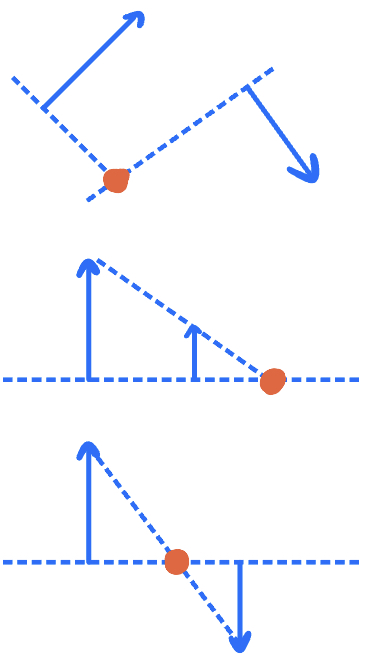
\includegraphics[width=0.18\textwidth]{CIR.jpeg}
\end{wrapfigure}

\phantom{\ \ \ }  Inoltre il CIR può anche essere fuori dal corpo rigido \\ \\
%
%
%
Teorema: \textbf{Chasles}\ \ \ (+dim)\\ 
\phantom{\ }La posizione del CIR in un atto di moto rigido piano si trova: \\
\ \ • \ all'intersezione delle rette perpendicolari a $\overline{v}_P \ e\ \overline{v}_Q$ passanti per P e Q \\
\ \ • \ sulla retta $\perp \ a \ \overline{v}_P /\!\!/ \overline{v}_Q$ t.c. $\frac{|\overline{v}_P|}{|\overline{CP}|} = \frac{|\overline{v}_Q|}{|\overline{CQ}|}$ \\
\pagebreak




\subsection{Cinematica Relativa}
%
%
Prop: \textbf{Trasformate di Galileo} (o legge di trasformazioni della velocità) \ \ \ (+dim)\\
\phantom{\ } $\exists$ matrice ortogonale $R\in\theta_3 \ t.c \ \overline{x}_P = R\overline{x}_P' + \overline{OO'}$ e un vettore $\overline{\omega} \in \mathbb{R}^3$ t.c. \\
\phantom{\ } $\overline{v}_P = \overline{v}_P' + \underline{ \overline{v}_{O'} + \overline{\omega} \wedge \overline{x}_P'}$ \ \ \ dove $\overline{v}_{O'}$  è velocità relativa e \underline{ \ \ }  è velocità di trascinamento \\ \\
%
%Lezione 6
%
Teorema: \textbf{Coriolis} \ \ \ (+dim)\\
\phantom{\ } Dati due osservatori $\theta \ e \ \theta'$ con accelerazione relativa $\overline{a}_{O'}$ e velocità angolare $\omega$, allora: \\
\phantom{} \hspace{1in} $\overline{a}_P=\overline{a}_P' +  \underline{\overline{a}_{O'} + \dot{\overline{\omega}}\wedge\overline{x}_P' +  \overline{\omega}\wedge(\overline{\omega}\wedge\overline{x}_P')} +  2\overline{\omega}\wedge\overline{v}_P'$ \\
\phantom{\ } dove \underline{ \ \ } è l'accelerazione di trascinamento, \ \ $\overline{\omega}\wedge(\overline{\omega}\wedge\overline{x}_P')$ è l'acc. centrifuga \ e \ $2\overline{\omega}\wedge\overline{v}_P'$ è l'acc. di Coriolis \\ \\
%
%
%
Oss: Affinché $\theta \ e\ \theta'$ abbiano le stesse accelerazioni $(\overline{a}_P = \overline{a}_P')$,  serve \ $\overline{a}_{O'}=\overline{\omega}=\dot{\overline{\omega}}=\overline{0} $ \\
\phantom{Oss: }allora $\theta \ e\ \theta'$ sono osservatori relativamente inerziali e sono in moto relativo rettilineo uniforme \\
%
%
Corollario: \textbf{Rivals} \ \ \ (+dim)

Dati P e Q di un corpo rigido si ha \ \ $\overline{a}_P=\overline{a}_Q + \dot{\overline{\omega}}\wedge\overline{QP} +  \overline{\omega}\wedge(\overline{\omega}\wedge\overline{QP})$ \\
%
%
Corollario: Dato un corpo rigido con $\overline{\omega}, \dot{\overline{\omega}}\neq\overline{0},$

$\exists! C$ \textbf{centro delle accelerazioni} t.c. $\overline{a}_C = \overline{0} \ e \ \forall P \in C \ \ \ \overline{PC} = \frac{  \dot{\overline{\omega}}\wedge\overline{a}_P - \overline{\omega}\wedge(\overline{\omega}\wedge\overline{a}_P) }{ \omega^4 + \dot{\omega}^2  } $ \\




\subsection{Moti e Atti di moto Rigidi}
%
%
%
Riassunto Moti piani:\\
\ • \ \ Traslatorio ha atto di moto traslatorio $\forall t$\\
\ • \ \ Rotatorio, Rototraslatorio, Polare hanno atto di moto rotatorio $\forall t$\\
Per gli atti di moto rotatorio piani abbiamo: $\begin{cases}
\overline{\omega}(t)=\dot{\theta}\hat{k} \\
\overline{V}_P=\overline{\omega}(t)\wedge\overline{CP}
\end{cases}$ \\ \\
%
%
%
Prop: Composizione velocità angolari \ \ \ (+dim)\\
\phantom{Prop: }Siano $\overline{\omega}_C, \ \overline{\omega}_C' \ e \ \overline{\omega}$ le velocità angolari di C rispetto a $\theta \ e\ \theta'$ e di $\theta'$ rispetto a $\theta$, allora: \ \ \ $\overline{\omega}_C = \overline{\omega}_C' + \overline{\omega}$ \\
Oss: Questa legge può essere utile per decomporre, con osservatori mobili, il moto in moti più semplici
%
%
%
\begin{wrapfigure}{r}{0.18\textwidth}
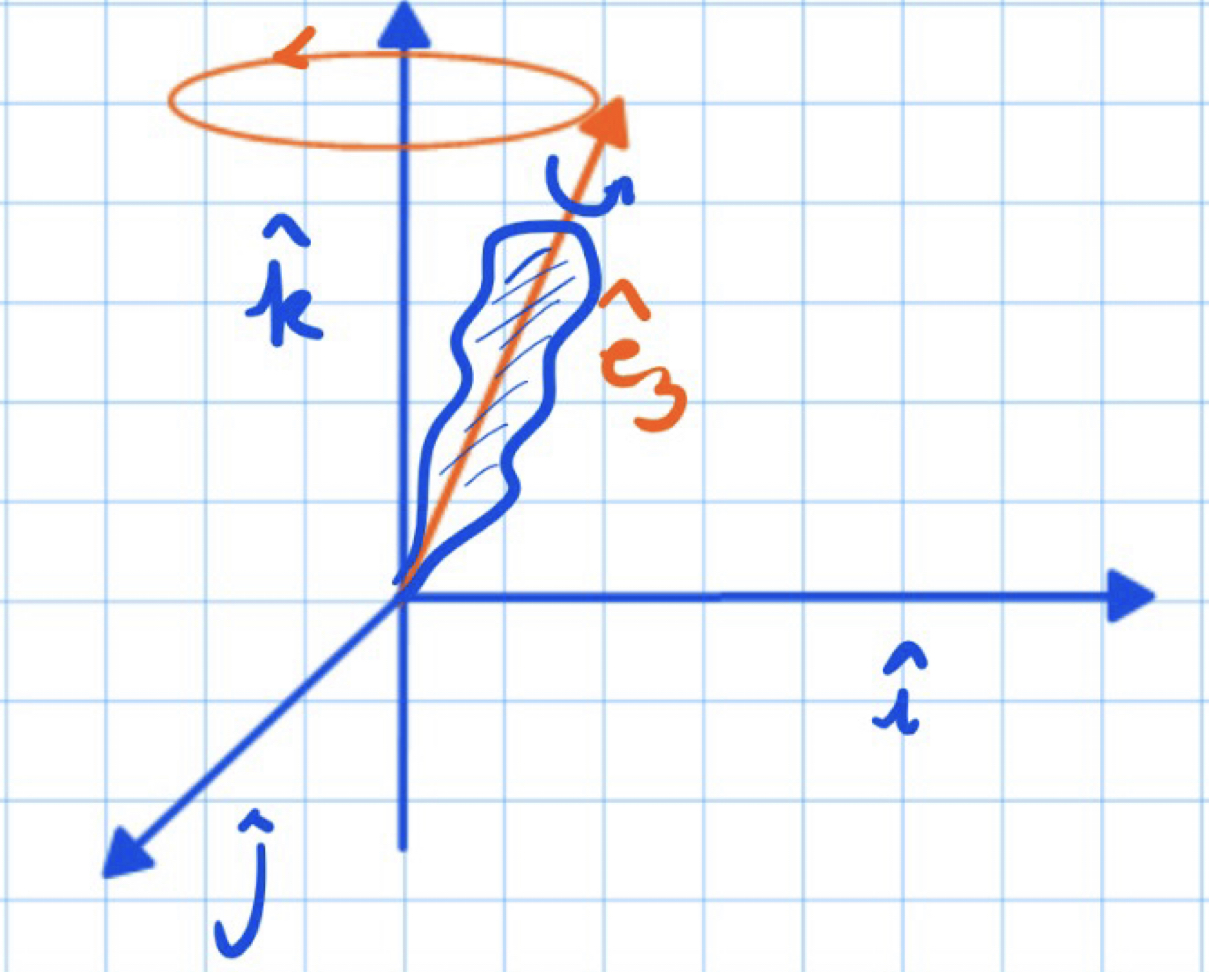
\includegraphics[width=0.2\textwidth]{Processionale.jpeg}
\end{wrapfigure} \\
%
Un moto di C è \textbf{Precessionale} se si possono scegliere $\theta \ e\ \theta'$ in modo che $\hat{e}_3\cdot\hat{k} = \ cost$

con $\hat{e}_3$ asse di rotazione propria e $\hat{k}$ asse di precessione \\
Prop: Un moto di C è una precessione $\Longleftrightarrow \overline{\omega}= \lambda(t)\hat{k}+\mu(t)\hat{e}_3$ \ \ \ (+dim) \\
\pagebreak


%
%Lezione 7
%
\subsection{Vincoli}
%
\textbf{Vincolo} è una restrizione delle possibili configurazioni, moti, atti di moto di un sistema di punti materiali. \\
Un vincolo è della forma $F(\overline{x}_1, ..., \overline{x}_N, \overline{v}_1, ... , \overline{v}_N, t ) \geq 0$ \ \ dove $F:\mathbb{R}^{dN}\times\mathbb{R}^{dN}\times\mathbb{R}\rightarrow\mathbb{R} \ t.c \ \ \ F \in C^\infty(\mathbb{R}^{2dN}\times\mathbb{R})$ \\
Oss: Ogni vincolo è uno scalare, noi quindi scriveremo un "vettore" di vincoli. \\ \\
%
%
%
I vincoli possono essere: \\
\ \ • \ \textbf{olonomo} se F non dipende dalle velocità \\
\ \ • \ \textbf{anolonomo} se F dipende dalle velocità \\
\ \ • \ \textbf{fisso} se F non dipende dal tempo\\
\ \ • \ \textbf{unilatero} se il vincolo è F(...) $\geq$ 0 \\
\ \ • \ \textbf{bilatero} se il vincolo è F(...) = 0 \\
Oss: Un vincolo anolonomo è integrabile se è equivalente a un vincolo olonomo \\ \\
%
%
%
Le \textbf{coordinate libere}, o Lagrangiane, sono un insieme minimale di parametri sufficiente a caratterizzare 

univocamente un sistema di punti materiali, Il \textbf{Grado di libertà} g è il numero di coordinate libere

Dati N punti materiali senza vincoli ottengo $g_0=dN$ gradi \\ \\
%
%
%
Varietà delle configuarazioni di un sistema vincolato (olonomi, bilateri) al tempo t è:

$\Sigma_t := \{ (\overline{x}_1, ..., \overline{x}_N) \in \mathbb{R}^{dN} \ t.c. \ \overrightarrow{F}(\overline{x}_1, ..., \overline{x}_N, t ) = 0 \}$ \\ \\
%
%
%
Dati M vincoli [ $\overrightarrow{F} = (F_1,...,F_M)$ ] olonomi e bilateri, si dicono:\\
\ \ • \ \textbf{compatibili} \ se $\Sigma_t \neq 0 \ \ \ \forall t \in \mathbb{R}$ \\
\ \ • \ \textbf{indipendenti}\ se $J_{ij}= \frac{\partial F_i}{\partial x_j} \implies rank(J_F)$ è massimo $\forall t \in \mathbb{R}$ \ \ \ \ allora $rank(J_F) = min \{ M,dN\} $ \\ \\
%
%
%
Teorema: Dato un sistema di $N\in\mathbb{N} \cup \{ +\infty \}$ punti materiali, sottoposto a M $\leq$ dN vincoli \\
\phantom{\ } Olonomi, bilateri, compatibili, indipendenti e fissato t, allora esistono: \\
\phantom{\ } $D_t$ (intorno di $\Sigma_t)\subset \mathbb{R}^{dN}$, \ \ un aperto $E_t\subset\mathbb{R}^g$ con g=dN-M, \\ 
\phantom{\ } Una funzione invertibile $\Phi : E_t \rightarrow D_t \ t.c. \ \ \Phi \in C^\infty(D_t)$ \ e \ $\overrightarrow{F}(\overrightarrow{\Phi}(\overline{q}),t) = \overline{0}$ \\
Oss: Questo teorema equivale alla generalizzazione a dN variabili del teorema della funzione implicita (Dini). \\ \\
%
%
%
Oss: Dato un sistema con $g_0$ gradi di libertà iniziali, dopo l'applicazione di M vincoli \\
\phantom{Oss: }Compatibili e indipendenti, avrò: \ \ \ \ \ \ \ \ $g=g_0-M$ \ (ovviamente se $g_0 \leq M$ avrò g=0) \pagebreak \\
%
%
%Lezione 8
%
Dato un punto materiale P, $\overline{v}_P'$ è una sua \textbf{velocità virtuale} se $(\overline{x}_P,\overline{v}_P')$ è un atto di moto possibile per P.

$\delta\overline{x}_P'$ è un suo \textbf{spostamento virtuale} se $\exists \delta t > 0 \ t.c. \ \delta\overline{x}_P' = \overline{v}_P'\delta t $

L'insieme delle velocità e spostamenti virtuali sono indicati con $V_P'(\overline{x}_P) \ e \ S_P'(\overline{x}_P)$ \ \ \ \ \ \ \ \ \ \ \
%
%
%
\begin{wrapfigure}{r}{0.32\textwidth}
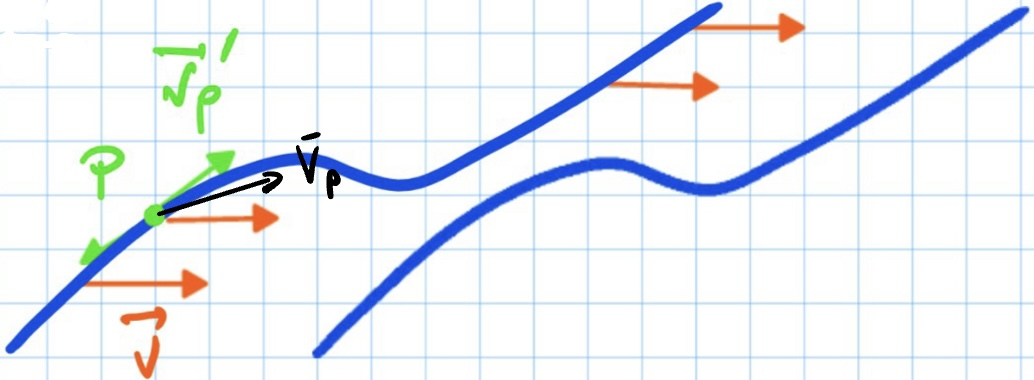
\includegraphics[width=0.32\textwidth]{Virtuali.jpeg}
\end{wrapfigure} \\
%
Oss: I valori virtuali dipendono dai vincoli.\\
Oss: A volte la velocità virtuale ha poco a che fare con quella reale \\
\phantom{Oss: }Per esempio quando il vincolo si muove ($\overline{v}$), abbiamo $\overline{v}_P = \overline{v}_P' + \overline{v}$  \ \\*
%
%
%
Le velocità virtuali sono \textbf{reversibili} se per ogni $\overline{v}_P'$ che è velocità virtuale, allora anche $-\overline{v}_P'$ lo è.

Vale lo stesso per gli spostamenti e gli spostamenti virtuali sono reversibili se e solo se lo sono le velocità.

Valori virtuali associati a vincoli bilateri sono sempre reversibili. \ \ \ \ \ \ \ \ \ \ \ \ \ \ \ \ \ \ \ \ \ \ \ \ \ \ \ \ \ \ \ \ \ \ \ 
%
%
%
%
\begin{wrapfigure}{l}{0.18\textwidth}
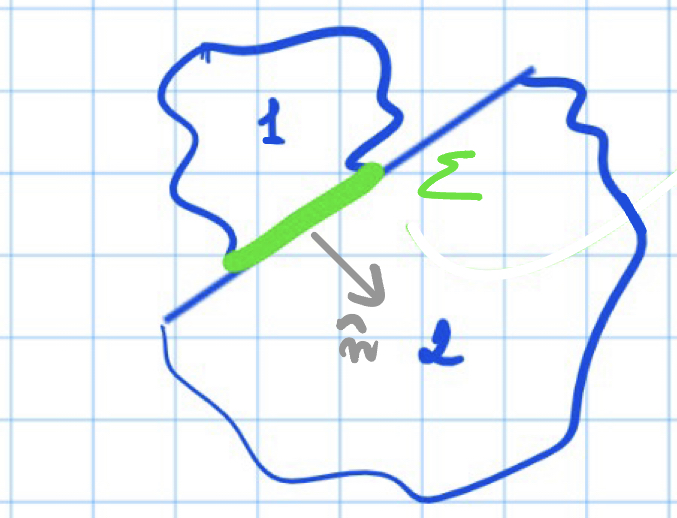
\includegraphics[width=0.18\textwidth]{Contatto.jpeg} \\ \\
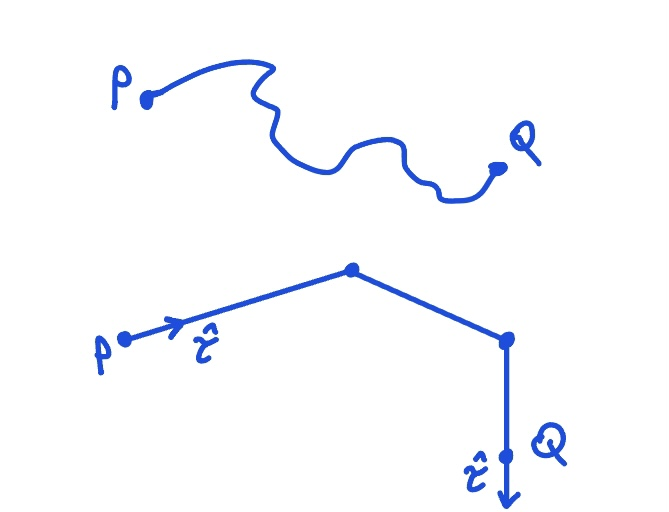
\includegraphics[width=0.18\textwidth]{Filo.jpeg}
\end{wrapfigure} \\
%
Vincoli anolonomi tra superfici $\Sigma$ \ \ (di contatto o di appoggio):\\
\textbf{contatto} \ (bilatero) \ \ \ $\overline{v}_{P_1}\cdot\hat{n} =\overline{v}_{P_2}\cdot\hat{n} \ \ \ \ \forall P \in \Sigma$ \\
\textbf{appoggio} (unilatero) \ $(\overline{v}_{P_1} -\overline{v}_{P_2})\cdot\hat{n} \leq 0 \ \ \forall P \in \Sigma$ \ (vincolo vale finchè c'è contatto) \linebreak \\ \\
%
%
Vincoli olonomi su un Filo:\\
\textbf{inestensibile} (unilatero) $|\overline{PQ}| \leq l$\\
\textbf{in tensione} \ (bilatero) $\overline{V}_P\cdot \hat{\tau} = \overline{V}_Q\cdot\hat{\tau} \ \ \forall P,Q$ nel filo \\ \\
%
%
%
\textbf{Puro Rotolamento} è un vincolo anolonomo e\\
\ • \ \ unilatero se disco è appoggiato $\overline{v}_P  \cdot \hat{j} \geq 0 \ \ \forall t \in \mathbb{R} \ t.c. \ y_P(t)=0$\\
\ • \ \ bilatero se disco è vincolato a rotolare sulla guida, quindi \ \ $y_P(t)=0 \ \forall t \in \mathbb{R}$

Inoltre abbiamo il vincolo $\overline{v}_{P_{disco}}=\overline{v}_{P_{guida}}$ \ \ (anche se i punti di contatto cambiano) \\
Oss: Se la guida è fissa $\overline{v}_P=0$\\
Oss: Essendo un corpo pinao $g_0=3$ e avendo i due vincoli (contatto e rotolalmento), otterremo g=1 \\
Oss: In ogni istante il punto P (di contatto) sarà il CIR e \ \  $\overline{x}_C(t)=\overline{x}_C(0) + R(\theta(t) - \theta(0))\hat{i}$ \\
Oss: In generale i vincoli di contatto possono essere di \textbf{strisciamento} se: $\overline{v}_{A_1} \cdot \hat{\tau} \neq \overline{v}_{A_2} \cdot \hat{\tau}$ \\ \\
%
%
%
Un \textbf{Sistema olonomo} è un sistema sottoposto a M vincoli bilateri, olonomi e fissi che assumeremo

Compatibili e indipendenti, allora avrà g = gradi di libertà = dN - M \\ \\
%
%
%
Per ogni sistema olonomo esistono delle coordinate libere $\overline{q} \in \mathbb{R}^g$, per le quali ho un cambiamento di base

Regolare e invertibile t.c. $\overline{x}=X(\overline{q})$ e $\overline{q}=Q(\overline{x})=X^{-1}(\overline{x})$ \\ \\
%
%
%
%Date $\dot{q}_j$ e $\ddot{q}_j$ velocità e accelerazioni generalizzate, abbiamo $\overline{v}_i(t)=\sum_{j=1}^g\frac{\partial\overline{x}_i}{\partial q_j}\dot{q}_j \ \ \overline{a}_i(t)=\sum_{j,k=1}^g\{ \}$



\section{Leggi della Dinamica}

Oss: A differenza della statica la dinamica dipenderà dalla scelta dell'osservatore
\subsection{Principi della Dinamica}
%
%
\textbf{I principio dinamica o principio d'Inerzia}\\
Esiste almeno un sistema (osservatore) di rifermento inerziale.

Oppure: Esiste una classe non vuota di sistemi inerziali in moto rettilineo uniforme (stesse accelerazioni) \\ \\
%
%
%
\textbf{II principio dinamica o legge di Newton}\\
Dato un punto materiale P e un osservatore inerziale, \ $\exists$ \ massa inerziale $m>0$, \ forza $\overline{F}\in\mathbb{R}^d$ \ t.c. \\
\phantom{} \hspace{2in} $m\overrightarrow{a}=\overrightarrow{F}$\\
%
%
Oss: Legge di Newton è \textbf{covariante}, cioè è invariante per cambiamento di osservatore inerziale ($\overline{a}=\overline{a}'$)

Infatti sia R il cambio di base, allora $m\overline{\ddot{x}}=\overline{F} \Leftrightarrow mR\overline{\ddot{x}}'=R\overline{F}'$ \\ \\
%
%
%
Oss: La Forza è una grandezza fisica data, non è definita da legge Newton \\
Oss: $\overline{F}$ è un vettore applicato, serve definire il punto di applicazione \ \ $(\overline{F},P)$\\
Oss: Posso anche definire $\overline{F}=\overline{F}(\overline{x},\dot{\overline{x}},t)$ con $\overline{F}:\mathbb{R}^d\times\mathbb{R}^d\times\mathbb{R}\rightarrow\mathbb{R}^d$ t.c. $(\overline{F} \in C^\infty)$

Questo equivale a un pb. di Cauchy di d equazioni differenziali del 2° ordine: \ \ \ \
$\begin{cases}
\ddot{\overline{x}}=\dfrac{1}{m}\overline{F}( \overline{x},\dot{\overline{x}},t) \\
\dot{\overline{x}}(0) =\overline{v}_{0}\\
\overline{x}(0) =\overline{x}_{0}
\end{cases}$ \\
Condizione di esistenza e unicità: $\overline{F}$ \ Lipschitz su $A\subset\mathbb{R}^{2d}$ (aperto, limitato) e continua in T (posto $t\in[0,T)$)\\
Oss: Condizione necessaria affinché $\overline{f}$ sia Lipshitziana in A aperto è che esistano finite tutte le derivate parziali \\ \\
%
%
%
Oss: In un sistema di riferimento non inerziale la forza $\overline{F}'$ segue dal II principio e teorema di Coriolis: \\
\phantom{} \hspace{0.5in}  $m\overline{a}'=\overline{F} - m\{\dot{\overline{\omega}}\wedge\overline{x}'  +  \overline{\omega}\wedge(\overline{\omega}\wedge\overline{x}')  +  2\overline{\omega}\wedge\dot{\overline{x}}'\}$ \ \ \ (ovvero F reale - forze apparenti) \\ \\
%
%
%
\textbf{III principio dinamica}\\
L'iterazione tra due punti materiali è data da due forze uguali e contrarie dirette lungo la congiungente: \\
\phantom{} \hspace{2in} $\overline{F}_1=-\overline{F}_2=f\frac{\overline{P_1P_2}}{|P_1P_2|}$ \\
Una \textbf{Coppia di forze} è data da due forze con stessa intensità, applicate a punti diversi: $(\overline{f},P) \ e \ (-\overline{f},P')$



%Lezione10

\subsection{Forze}
%
Tipi di Forze $\overline{F}(\overline{x}, \dot{\overline{x}},t)$:\\
\ • \ \ \textbf{interna} se dovuta dall'interazione con altri punti del sistema (III principio)\\
\ • \ \ \textbf{esterna} altrimenti \\
\ • \ \ \textbf{costante} se $\overline{F} = \overline{F}_0 \in \mathbb{R}^d$\\
\ • \ \ \textbf{posizionale} se $\overline{F} = \overline{F}(\overline{x})$\\
\ • \ \ \textbf{centrale} se è posizionale ed $\exists O \in \mathcal{E}_d$ (centro) \ t.c. $\overline{F}(\overline{x})=f(|\overline{x}-\overline{x}_0|)\cdot \frac{\overline{x}-\overline{x}_0}{|\overline{x}-\overline{x}_0|}$\\ \\
%
%
%
Data una forza posizionale $\overline{F}(\overline{x})$ e una curva $\Gamma$ parametrizzata da $\overline{\gamma}:[s_0,s_1]\rightarrow\mathbb{R}^d$\\
Il \textbf{Lavoro} compiuto da $\overline{F}$ lungo $\Gamma$ è \ \ \ $L=\int^{s_1}_{s_0} \overline{F}(\overline{\gamma}(s))\cdot\overline{\gamma}'(s)ds$ \\ \\
%
%
%
Oss: Il lavoro infinitesimo di $\overline{F}$ in $d\overline{x}$ è $dL = F_1dx_1 + F_2dx_2+ F_3dx_3$ cioè una 1-forma differenziale\\
%
Una 1-forma differenziale è $\omega=\sum_{j=1}^3 f_j(\overline{x})dx_j$ e in A aperto di $\mathbb{R}^3$ è:\\
\ • \ \ \textbf{esatta}  se $\exists g:A\rightarrow\mathbb{R}^3, g\in C^1(A) \ t.c. \ \ \omega = dg = \sum_{j=1}^3 \frac{\partial g}{\partial x_j} \ dx_j$ \\
\ • \ \ \textbf{chiusa} se $d\omega=0$ dove $d\omega= \sum_{j=1}^3 \partial F_j \wedge dx_j$ \\
%
Oss: La forma differenziale del lavoro in un dominio semplicemente connesso A è esatta  $\ \Leftrightarrow \ \frac{\partial F_i}{\partial x_j}=\frac{\partial F_j}{\partial x_i} \ \ \forall \overline{x}\in A$\\
%
Oss: Se dL è esatta e $\overline{F}\in C^1(A) \implies \frac{\partial F_i}{\partial x_j}=\frac{\partial F_j}{\partial x_i}$ in A \\ \\
%
%
%
Teo: Ogni forma $\omega$ esatta è anche chiusa, ovvero $d^2\omega = 0$\\
Teo: In un aperto semplicemente connesso di $\mathbb{R}^n$ ogni 1-forma differenziale chiusa è anche esatta\\ 
%
Prop: Se la forma dL è esatta $\implies \int_{\Gamma_0} dL = 0 \ \ \ \forall \ \Gamma_0$ curva chiusa \ \ \ (+dim)\\ 
%
Teo: Condizione necessaria affinché dL sia esatta è che $\overline{F}$ sia posizionale\ \ \ (+dim)\\ \\
%
%
%
$\overline{F}$ posizionale è \textbf{conservativa} in $A\subset\mathbb{R}^3$ \ \ se $\exists$ \textbf{potenziale} $U\in C^2(A) \ t.c. \ \ \overline{F}(\overline{x})=-\nabla U(\overline{x})$\\
Teo: In A aperto semplicemente connesso di $\mathbb{R}^3 \ \ \ \overline{F}$ posizionale e conservativa $\Leftrightarrow \ \nabla \wedge \overline{F} = \overline{0}$ \ \ \ (+dim)\\
\phantom{} \hspace{0.23in} dove $(\nabla\wedge\overline{F})_i = \sum^3_{j,k=1} \varepsilon_{ijk} \frac{\partial}{\partial x_j}F_k$ \\ \\
%
%
%
Una forza $\overline{F}$ si dice \textbf{attiva} se è nota a priori la sua dipendenza da $\overline{x}, \dot{\overline{x}}$ e t\ \ cioè $\overline{F}=\overline{F}(\overline{x},\dot{\overline{x}},t)$ \\
In ogni altro caso di dice \textbf{reazione vincolare} $\overline{\Phi}$ \ ed è dovuta dalla presenza di un vincolo\\
%
Oss: La legge di Newton si può riscrivere: \ \ $m\overline{a} = \overline{F}^{(att)} + \overline{\Phi}$ \\ \\
%
% 
%
Esempi di forze e potenziali:\\
\ • \ \ Forza \textbf{peso} è una forza costante, $\overline{F}_g=m\overline{g}$ \ con $\overline{g}=-g\hat{j}$\\
\phantom{} \hspace{0.18in} Le forze costanti sono conservative con $U(\overline{x})=-\overline{F}_0\cdot\overline{x}$ \hspace{0.18in} per $\overline{F}_g: \ \ U_g(\overline{x})= mgy$\\
%
\ • \ \ Forza \textbf{elastica} è una forza posizionale, $\overline{F}_{el}(\overline{x})=-k(\overline{x}-l)\hat{x}$ \hspace{0.18in} $U_{el}(\overline{x})=\frac{1}{2}k(|\overline{x}|-l)^2$\\
%
\ • \ \ Forza \textbf{gravitazionale} è una forza posizionale, $\overline{F}_{1,2} = -G\frac{m_1m_2}{r^2}\hat{r} \ \ \ (\overline{r}=\overline{x}_1 - \overline{x}_2$)\\
\phantom{} \hspace{0.18in} Se $m_2=M>>m=m_1$ allora diventa una forza centrale in $\overline{x}_2$ \ \ e avremo $f(\overline{r}) = \overline{F}_{1,2}(\overline{x}_1 , \overline{x}_2)$\\
\phantom{} \hspace{0.18in} Le forze centrali sono conservative con $U(\overline{r})=g(|\overline{r}|)$ dove g è la primitiva di $-f(\overline{r})$ \hspace{0.12in} $U_G(\overline{r})= -\frac{GMm}{r}$\\






\section{Statica}
%
%
%
\subsection{Equazioni Cardinali della Statica}
%
Le equazioni del moto $\overline{F}=m\overline{a}$ per un punto materiale ammettono la \textbf{soluzione di Quiete} in $\overline{x}_0\in\mathbb{R}^d$\\
\phantom{\ \ \ \ } se $\overline{x}(t)=\overline{x}_0, \forall t \in \mathbb{R}$ è soluzione delle eq. stesse\\
%
Un sistema di N punti materiali sottoposto alle forze $\{\overline{F}_j(\overline{x}_1,...,\overline{x}_N,\overline{v}_1,...,\overline{v}_N,t)\}$\\
\phantom{\ \ \ \ } Ha una \textbf{configurazione di equilibrio} $\{\overline{x}_{j\in\{1...N\}}^{(0)}\}$ \ \ \ se \
$\overline{F}_j(\overline{x}_1^{(0)},...,\overline{x}_N^{(0)},\overline{0},...,\overline{0},t)=\overline{0} \ \ \forall t,j$ \\
%
Oss: Se la forza è Lipschitz, $\{\overline{x}_{j\in\{1...N\}}^{(0)}\}$ è soluzione di quiete se e solo se è configurazione di equilibrio \\
Oss: Le forze si possono sempre scomporre: \ \
$\overline{F}_j=\overline{F}_j^{(ext)}+\overline{F}_j^{(int)}=\overline{F}_j^{(att)}+\overline{\Phi}_j$ \\ \\
%
%
%
Data una forza $(\overline{f},\overline{x}_P)$ applicata in P, il suo \textbf{Momento} rispetto al \textbf{polo} O è $\overline{m}=(\overline{x}_P-\overline{x}_O)\wedge\overline{f}$\\
\phantom{\ \ \ \ } Avremo $|\overline{m}|= |\overline{OP}||\overline{f}||sen\theta|$ \ e \ $\overline{m}=m \ \hat{k}$ \\
%
Un \textbf{sistema di forze} \ $\mathcal{S}=\{(\overline{f}_1,\overline{x}_1),...,(\overline{f}_n,\overline{x}_n)\}$ è una collezione di vettori applicati \\
La \textbf{Risultante} e il Momento risultante di $\mathcal{S}$ rispetto a O sono: \ \ $\overline{R}=\sum_{j=1}^n\overline{f}_n \ \ \ \overline{M}_O=\sum^n_{j=1}(\overline{x}_j-\overline{x}_0)\wedge\overline{f}_j$ \\ \\
%
%Lezione11
%
Teorema: Condizione necessaria per un sistema meccanico in configurazione di equilibrio è che il sistema \\ \phantom{\ } di forze esterne rispetti le \textbf{equazioni cardinali della statica:} $\ \ \overline{R}^{(ext)}=\overline{0}, \ \ \overline{M}_O^{(ext)}=\overline{0} \ \ \forall O \in \mathcal{E}_3$ \ \ \ (+dim)\\
%
Lemma: Per ogni sistema meccanico il sistema di forze interne ha: $\ \ \overline{R}^{(int)}=\overline{0}, \ \ \overline{M}_O^{(int)}=\overline{0} \ \ \forall O \in \mathcal{E}_3$ \ \ \ (+dim)\\ \\
%
%
%
Oss: Dato un sistema in una conf di eq, le equazioni cardinali valgono anche per i suoi sottosistemi\\
%
Prop: Trasporto del momento \ \ \ (+dim)\\
\phantom{Prop: }Dato un sistema di forze $\mathcal{S}$ e due poli O, O' $\in \mathcal{E}_d$ si ha: $\overline{M}_{O'}=\overline{M}_O + \overline{OO'}\wedge\overline{R}$





\subsection{Sistemi di Forze}
%
Due sistemi di forze $\mathcal{S}, \mathcal{S}'$ si dicono \textbf{equivalenti} $\mathcal{S} \sim \mathcal{S}'$ \ se $\overline{R}=\overline{R}' \ e \ \overline{M}_O=\overline{M}_O' \ \forall O \in \mathcal{E}_3$ \\
%
%
Oss: L'equivalenza tra sistemi di forze è una relazione di equivalenza, cioè valgono le proprietà:\\
\phantom{Oss: }i) riflessiva: $\mathcal{S} \sim \mathcal{S}$ \ \ \ ii) simmetrica: $\mathcal{S} \sim \mathcal{S}' \Leftrightarrow \mathcal{S}' \sim \mathcal{S}$ \ \ \ iii) transitiva: $\mathcal{S} \sim \mathcal{S}' \ e \ \mathcal{S}' \sim \mathcal{S}'' \implies \mathcal{S} \sim \mathcal{S}''$ \\ \\
%
%
%
L'\textbf{invariante scalare} di $\mathcal{S}$ rispetto a O è \ $I=\overline{R}\cdot\overline{M}_O$ \ \ \ I non dipende dal polo scelto\\
%
%
Prop: Dato $\mathcal{S}$ con $\overline{R}\neq \overline{0}, \ \exists h$ retta dell'\textbf{asse centrale} t.c. \ $\overline{M}_P /\!\!/ \overline{R} \ \ \forall P\in h$ \ \ e $h: \overline{x}=\lambda\overline{R}+\frac{\overline{R}\wedge\overline{M}_A}{|\overline{R}|^2} + \overline{x}_A$\\
\phantom{Prop: }con $A\in \mathcal{E}_3$ qualsiasi \phantom{\ \ \ } E se I=0, h è detto asse di applicazione della risultante e $\overline{M}_P=\overline{0}$ \ \ \ (+dim)\\ \\
%
%
%
Prop: Ogni sistema di forze è equivalente al più a una forza più una coppia di forze. \ \ \ (+dim)\\
%
Teo: Dato un sistema di forze $\mathcal{S}$ si ha uno dei seguenti casi: \ \ \ (+dim)\\
\phantom{\ \ \ \ \ \ } i) $\overline{R}=\overline{0}, \ \overline{M}_O=\overline{0} \Leftrightarrow \mathcal{S}\sim\emptyset$ \hspace{0.77in}
ii) $\overline{R}=\overline{0}, \ \overline{M}_O\neq\overline{0} \Leftrightarrow \mathcal{S}\sim$ coppia di forze \\
\phantom{\ \ \ \ \ \ } iii) $\overline{R}\neq\overline{0}, \ I=\overline{0} \Leftrightarrow \mathcal{S}\sim\{(\overline{R},P)\}, P\in h$ \ \ \ \ \
iv) $\overline{R}\neq\overline{0}, \ I\neq\overline{0} \Leftrightarrow \mathcal{S}\sim\{(\overline{R},O),(\overline{f},O),(-\overline{f},P)\}$ \\
%
Lemma: Siano $\mathcal{S}, \mathcal{S}'$ t.c. $\overline{R}=\overline{R}' \ e \ \overline{M}_O=\overline{M}_O'$ per un centro $O \in \mathcal{E}_3 \Leftrightarrow \mathcal{S} \sim \mathcal{S}'$ \ \ \ (+dim)\\ \\
%Oss: Per verificare l'equivalenza è sufficiente $\overline{R}=\overline{R}' \ e \ \overline{M}_O=\overline{M}_O'$ per un singolo O (trasporto del momento) \\ \\
%
%
%
Per un sistema di punti il \textbf{centro di massa} è $\overline{x}_{cm}=\frac{1}M \sum_{j=1}^Nm_j\overline{x}_j$ e $M=\sum_{j=1}^Nm_j$ è la massa totale \\
%
Per un sistema continuo $\exists \rho :\mathbb{R}^3\rightarrow\mathbb{R}^+$ detta distribuzione di massa t.c. \ $m_A=\int_A\rho(\overline{x})d\overline{x}$ è la massa in A\\
\phantom{\ \ \ \ } Allora \  $M=\int_{\mathbb{R}^3}\rho(\overline{x})d\overline{x}$ \ \ e \ \ $\overline{x}_{cm}=\frac{1}M \int_{\mathbb{R}^3} \overline{x}\rho(\overline{x})d\overline{x}$ \\
%
%
Oss: La forza peso applicata a un sistema è equivalente alla forza $\overline{F}_P=M\overline{g}$ applicata nel centro di massa
%
%Lezione 12
%
\subsection{Vincoli Ideali}
%
Dato un punto materiale con velocità $\overline{v}$, la \textbf{potenza istantanea} generata dalle forze $\overline{F}$ è $\Pi=\overline{F}(\overline{x},\overline{v},t)\cdot \overline{v}$ \\
%
Dato un moto $\overline{\gamma}(t):\mathbb{R}\rightarrow\mathbb{R}^3$ di un punto soggetto a $\overline{F}(\overline{x},\overline{v},t)$, allora il lavoro è:\\
\phantom{}\hspace{2in} $L \ =\ \int^{t_1}_{t_0} \dot{\overline{\gamma}}(\tau)\cdot\overline{F}(\overline{\gamma}(\tau),\dot{\overline{\gamma}}(\tau),\tau)\ d\tau \ = \ \int\Pi(\tau)d\tau$ \\ \\
%
%
%
Dato un sistema di punti $P_j$ sottoposti alle forze $\overline{F}_j$, il \textbf{lavoro} e la \textbf{potenza virtuali} sono le quantità:\\
\phantom{\ \ \ } $\delta L'=\sum^N_{j=1}\overline{F}_j\cdot\delta x_j' \ con \ \delta x_j' \in S_j' \ \ \forall j \in \{ 1...N\}$
\ \ \ \ $\Pi'=\sum^N_{j=1}\overline{F}_j\cdot v_j' \ con \ v_j' \in V_j' \ \ \forall j$ \\ \\
%
%
%
I vincoli a cui è sottoposto un sistema di punti sono \textbf{ideali} se generano \underline{tutte e sole} le reazioni vincolari \ \ \ \ \
\phantom{\ \ \ } $\{\overline{\Phi}_j\}_{j\in\{1...N\}}$ che producono lavoro virtuale o potenza virtuale non negative \\
\phantom{\ \ \ } Ovvero \ \ \ $\sum^N_{j=1}\overline{\Phi}_j\cdot\delta x_j'\geq 0 \ \ \forall \delta x_j' \in S_j' \ \forall j$ \ \ oppure se \ \ \ $\sum^N_{j=1}\overline{\Phi}_j\cdot v_j'\geq 0 \ \ \forall v_j' \in V_j' \ \forall j$ \\
Oss: Un vicolo \textbf{perfetto} è un vincolo ideale e bilatero \ \ (al posto del $\geq$ c'è =)\\
\phantom{Oss: }Un vicolo è liscio se non produce attrito e quindi la reazione vincolare è $\perp$ alla superficie di contatto \\
Oss: Tutti i vincoli che useremo sono ideali: incastro, cerniera, manicotto, carrello, \\
\phantom{Oss: }puro rotolamento, filo in tensione, guida e appoggio in assenza di attrito \\ \\
%
%
%
%\subsection{Principio dei lavori virtuali}
%
Un'\textbf{equazione pura} caratterizza la statica e la dinamica di un sistema e non contiene reazioni vincolari\\
%
%
%
Teorema: \textbf{Principio dei lavori virtuali PLV} \ \ \ (+dim)\\
\phantom{\ } Dato un sistema di punti sottoposto a vincoli ideali e \underline{fissi} la configurazione $\{P-j^{(0)}\}_{j\in\{1...N\}}$ è di equilibrio\\ \phantom{\ \ } se e solo se \ $\delta L'^{(att)}=\sum^N_{j=1}\overline{F}_j^{(att)}\cdot \delta \overline{x}_j'\leq 0 \ \ \  \forall\delta\overline{x}_j'\in S_j' \ \ \ \forall j$ \ \ \ (per vincoli perfetti c'è = invece di $\leq$)


%Lezione13

\subsection{Statica dei Sistemi Olonomi}
%
Siano: g= $\#$g.d.l. \ \ $\overline{q}$= coordinate libere \ \ $\overline{X}(\overline{q})$ fornisce coordinate originali in funzione di quelle libere.

Gli spostamenti virtuali  $ \delta \overline{x}_j' = \sum_{i=1}^g \frac{\partial \overline{x}_j}{\partial q_i}\cdot \delta q_i'$ \ \ (analogo per velocità virtuali)\\ \\
%
%
%
Prop: Lavoro virtuale delle forze attive per sistema olonomo è \ $\delta L'^{(att)}=\sum_{k=1}^gQ_k\delta q_k'$ \\ 
\phantom{Prop: }Dove $Q_K$ sono le componenti generalizzate delle forze attive \ \ $Q_k = \sum_{j=1}^N\overline{F}_j^{(att)}\frac{\partial\overline{x}_j}{\partial q_k}$ \ \ \ (+dim) \\
%
%
%
Prop: Un sistema olonomo è in equilibrio in $\overline{q}^{(0)} \ \Leftrightarrow \ Q_k(\overline{q}^{(0)})=0 \ \ \forall k \in \{1...g\}$ \ \ \ (+dim) \\ \\
%
%
%
Oss: Se le forze attive sono conservative, cioè $\exists \widetilde{U}:\mathbb{R}^{dN}\rightarrow\mathbb{R} \ t.c. \ \overline{F}_j^{(att)}=-\nabla_j\widetilde{U}(\overline{x}_1,...,\overline{x}_N)$, \\
\phantom{Oss: }Si definisce il potenziale in funzione delle coordinate generalizzate \ \ $U(\overline{q})=\widetilde{U}(\overline{x}_1(\overline{q}),...,\overline{x}_N(\overline{q}))$ \\
Teo: Sistema olonomo con forze attive conservative è in equilibrio in $\overline{q}(0) \ \Leftrightarrow \ \frac{\partial U}{\partial q_k}(\overline{q}^{(0)})=0 \ \ \forall k$ \ \ \ (+dim)\\ \\
%
%
%
Per un sistema olonomo avremo \textbf{configurazioni ordinarie} se $\overline{q} \in \Sigma^0$ (parte interna) \\
\phantom{} \hspace{0.25in} \textbf{Di confine} se $\overline{q} \in \partial\Sigma$ dove $\Sigma$ è lo spazio delle soluzioni ammissibili \ \ (serve per vincoli unilateri)\\
%
Oss: Lo spazio degli spostamenti virtuali cambia in base al tipo di configurazione: \ \ $S'(\overline{q}) = \begin{cases}\mathbb{R}^g \ se \ \overline{q} \in \Sigma^0 \\ \neq\mathbb{R}^g \ se \ \overline{q} \in \partial\Sigma \end{cases} $ \\
%
Prop: Una configurazione $\overline{q}^{(0)}$ ordinaria è di equilibrio \ $\Leftrightarrow \ Q_k(\overline{q}^{(0)})=0 \ \forall k$ \\
\phantom{Prop: }Una $\overline{q}^{(0)}$ è di confine allora $\exists \tilde{k} \in \{1...g\} \ t.c. \ \delta q_{\tilde{k}}'\geq 0$ oppure $\delta q_{\tilde{k}}'\leq 0$ \\
\phantom{Prop: }Inoltre $\overline{q}^{(0)}$ è di equilibrio $\Leftrightarrow \begin{cases}
Q_k(\overline{q}^{(0)})=0 \ \forall k \ t.c. \ \delta q_k' \in \mathbb{R} \\
Q_k(\overline{q}^{(0)})\geq 0 \ \forall k \ t.c. \ \delta q_k' \leq 0 \\
Q_k(\overline{q}^{(0)})\leq 0 \ \forall k \ t.c. \ \delta q_k' \geq 0
\end{cases}$ 



\subsection{Statica del Corpo Rigido}
%
Prop: Un copro rigido sottoposto a $\mathcal{S}^{(ext)}$, vale: \  $\delta L' = \overline{R}^{(ext)}\cdot\delta\overline{x}_C' + \overline{M}_C^{(ext)}\cdot\overline{\varepsilon} $ \ \ con $\overline{\varepsilon}=\overline{\omega}\delta t \in \mathbb{R}^3$ \ \ \ (+dim)\\
Prop: Per un corpo rigido con vincoli ideali e fissi \ \ equazioni cardinali $\Leftrightarrow$ configurazioni di equilibrio \ \ \ (+dim)\\ \\
%
%
%
Il \textbf{Poligono di appoggio} di un corpo rigido appoggiato su un piano $\Pi$ in un numero finito di punti è

l'unico poligono t.c. \ \ \ i) ogni vertice è un punto d'appoggio (non viceversa) \ ii) il poligono è convesso  \\
\phantom{} \hspace{1.51in} iii) i punti di appoggio che non sono vertici, non sono esterni al poligono \\
%
Prop: Un corpo rigido appoggiato è in equilibrio \ $\Leftrightarrow$ \ la proiezione di G su $\Pi$ è dentro al poligono \ \ \ (+dim)\\
%
%Lezione14
%
\newpage












\end{document}